\documentclass[12pt]{phage3slides} %

\title[CPT Annotation Infrastructure]{CPT Annotation Infrastructure}
\authorErasche{}

\begin{document}
\frame{\titlepage}

\section{Data Analysis}
\begin{frame}{Data Analysis for Genome Annotation}
	\begin{itemize}
		\item Sequencing Data
		\item Assembly to Contigs
		\item Structural Prediction
		\item Functional Prediction
		\item Publishing
	\end{itemize}
\end{frame}


\subsection{Galaxy}
\begin{frame}{Galaxy for Reproducible Genomics}
	\begin{itemize}
		\item Standard interface to huge variety of tools
		\item ``Histories'' (audit logs) for later reference
		\item Workflows for sharing complex, multi-step analyses
		\item Collaboration between developers and end users
	\end{itemize}
\end{frame}

{%
  \usebackgroundtemplate{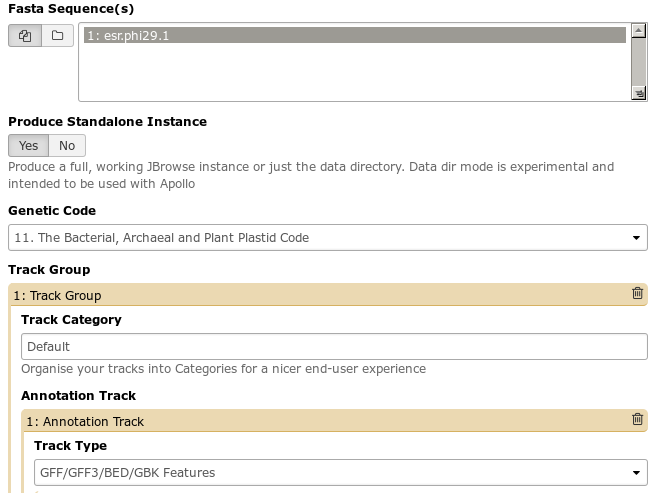
\includegraphics[height=\paperheight,width=\paperwidth]{gx-tool.png}}
  \setbeamertemplate{navigation symbols}{}
  \begin{frame}[plain]
  \end{frame}
}

{%
  \usebackgroundtemplate{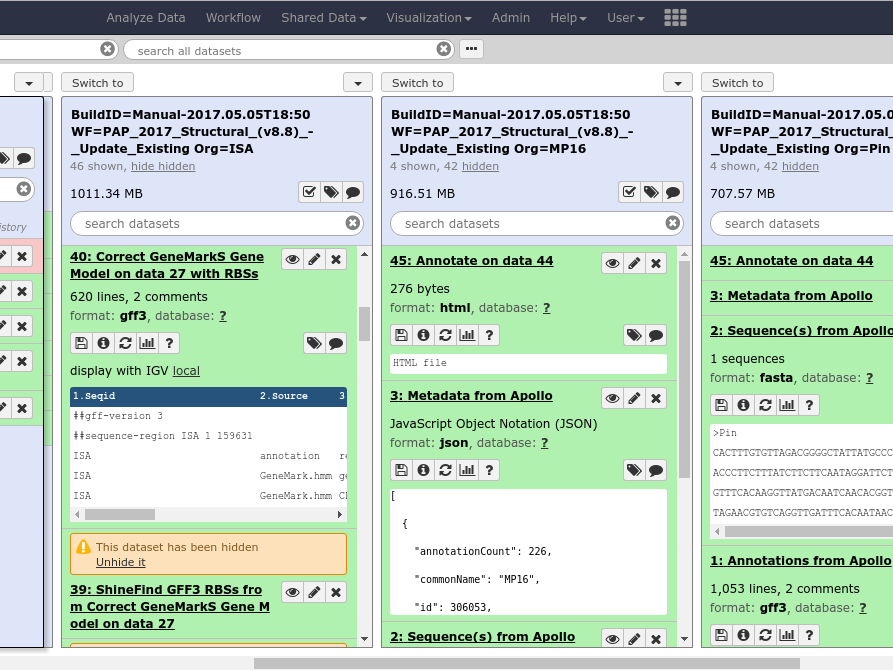
\includegraphics[height=\paperheight,width=\paperwidth]{history.png}}
  \setbeamertemplate{navigation symbols}{}
  \begin{frame}[plain]
  \end{frame}
}

{%
  \usebackgroundtemplate{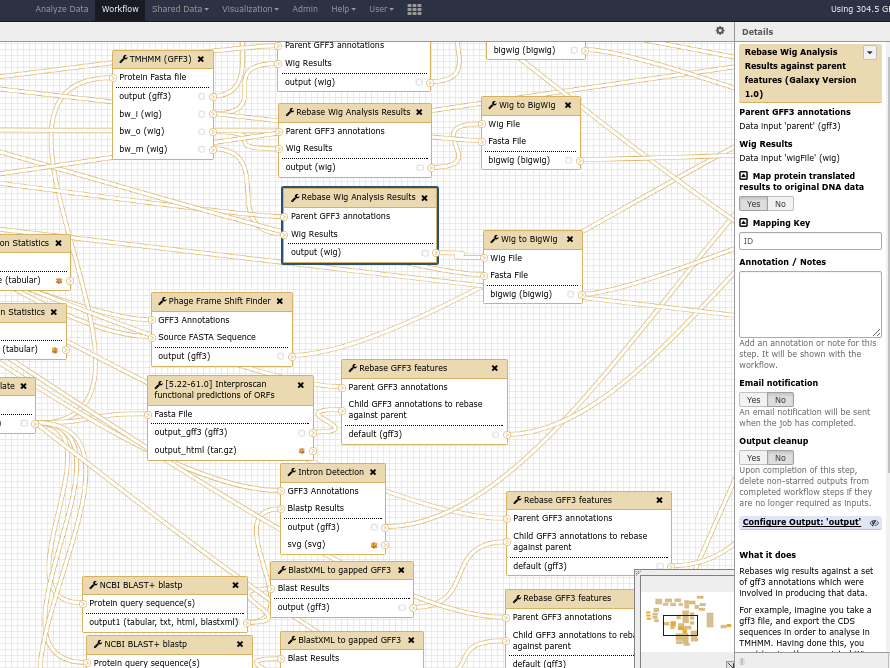
\includegraphics[height=\paperheight,width=\paperwidth]{workflows.png}}
  \setbeamertemplate{navigation symbols}{}
  \begin{frame}[plain]
  \end{frame}
}

\subsection{Apollo}
\begin{frame}{Apollo for Interactive Annotation}
	\begin{itemize}
		\item ``Google Docs'' for genome annotation
		\item Standard interface to analysis data
		\item Rapidly evolving service with a bright future
	\end{itemize}
\end{frame}

{%
  \usebackgroundtemplate{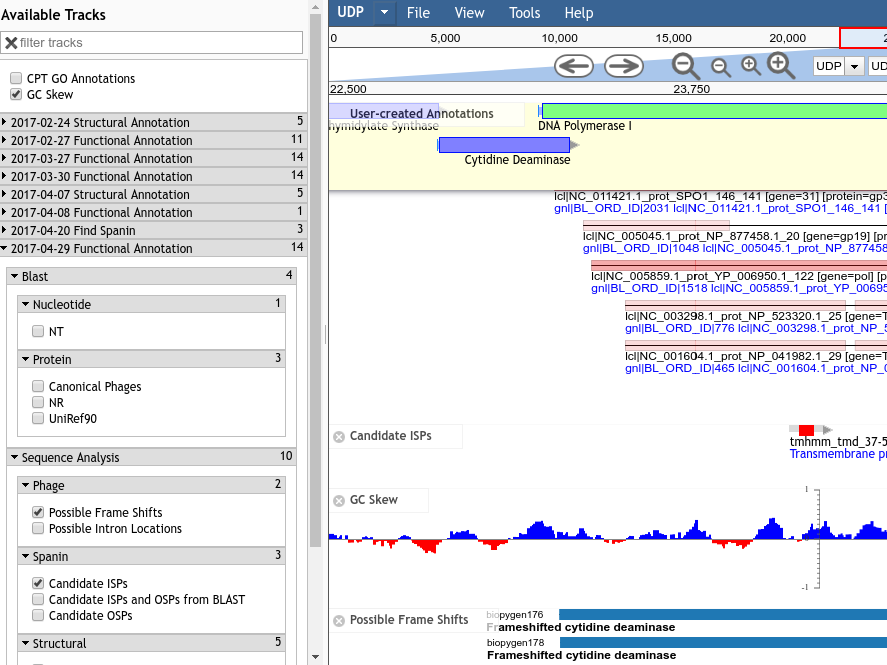
\includegraphics[height=\paperheight,width=\paperwidth]{apollo.png}}
  \setbeamertemplate{navigation symbols}{}
  \begin{frame}[plain]
  \end{frame}
}

\section{Summary}
\begin{frame}{Phage Genomics with CPT Galaxy \& Apollo}
	\begin{itemize}
		\item Full-spectrum platform, \emph{sequencing to publishing}
		\item \emph{Collaboration}, genome annotation and analysis
		\item \emph{Reproducible} science
	\end{itemize}
\end{frame}

\informationErasche%

\end{document}
